
%% ~1 page

\section{Introduction}
In recent years society has undergone a digital transformation and our everyday life depends on digital technology more than ever before. This development relies on an ever-growing collection of software systems and services that span our society and connect our lives. With the increasing size and scope of these software projects, and the growing numbers of software developers working in the same project simultaneously, the complexity of the source code can become a large problem. It is hard for stakeholders to get an overview of how the project in general, and more specifically the source code, evolves over time.

Today, it is common for software development teams to work according to an agile methodology \cite{hazzan_agile_2014} where requirements and solutions in a project are evolving over time in collaboration between developers, project managers and users. This process is conducted in an iterative cycle with continuous reflections and improvements on previous work.

In order to handle these iterative and fast paced change to the source code in a project, development teams are using a version control system to keep track of changes. Based on search trends on \textit{Google}\footnote{https://trends.google.com} displayed in figure \ref{fig:vcstrends}, the most used tool for software version control is \textit{Git}\footnote{https://git-scm.com/}, a system where developers can commit incremental changes to the code and collaborate on different versions of the source code in parallel. All these small incremental changes are recorded and make up a rich source of information into the evolution of the code. However, this information is cumbersome to grasp and oversee and therefore often not used in an effective way.

\begin{figure}[b]
  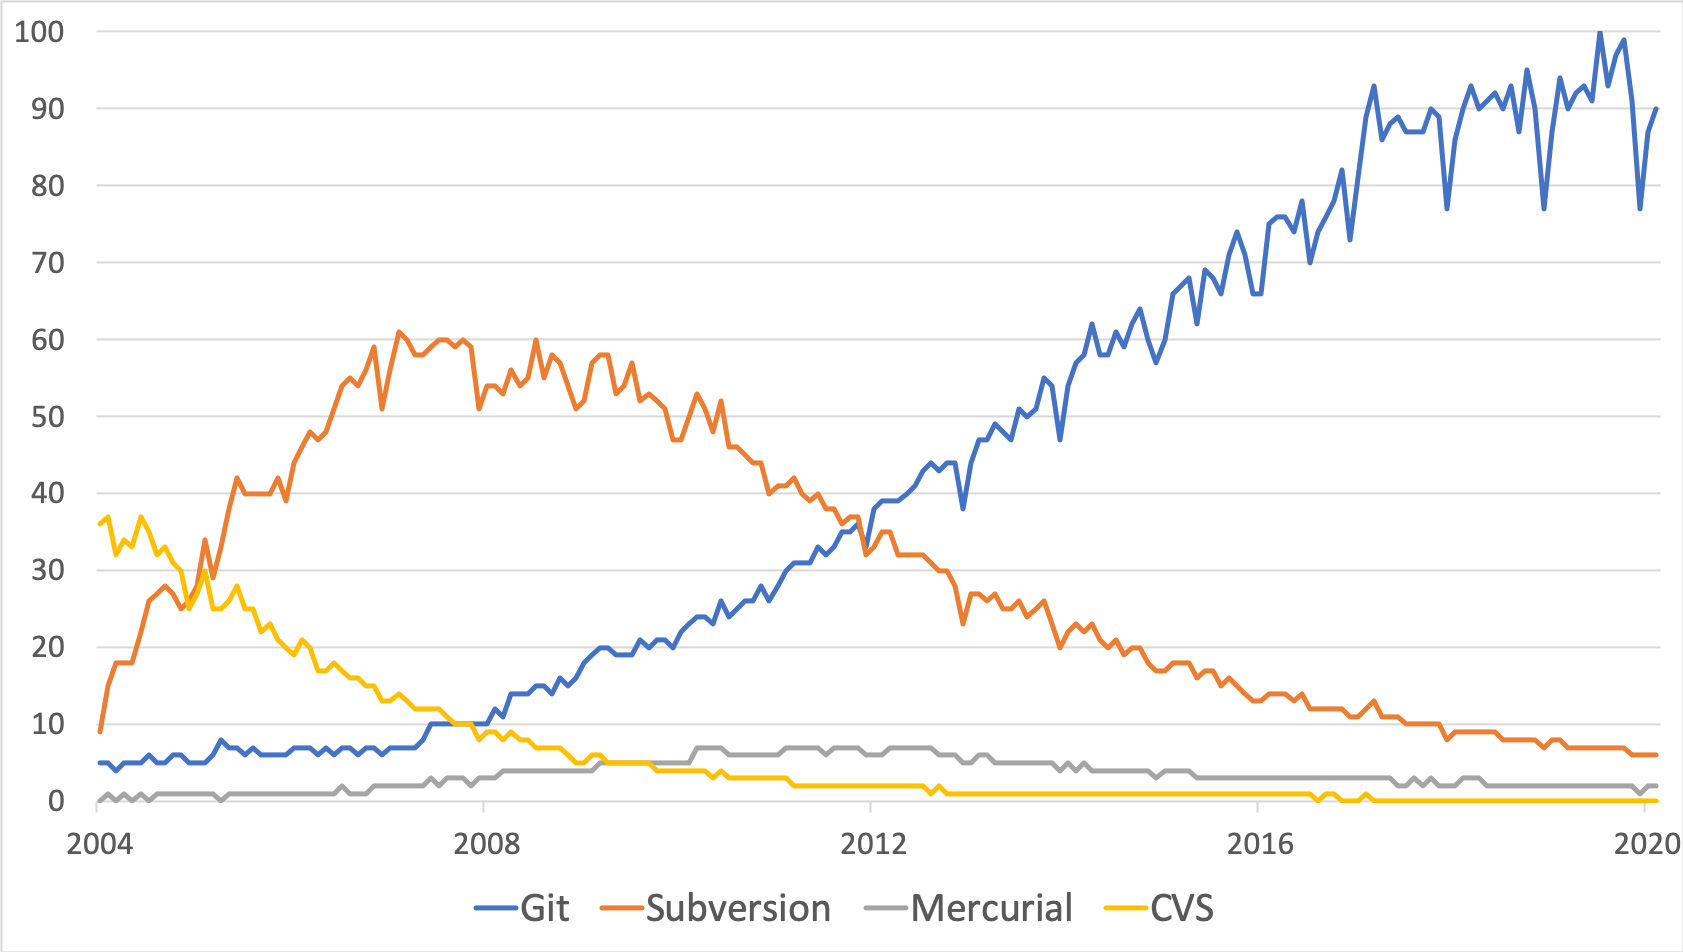
\includegraphics[width=\columnwidth]{VCSTrends}
  \caption[VCS Trends]{Popularity of version control systems 2004-2020}
  \label{fig:vcstrends}
  \centering
\end{figure}

In this context, where rapid continuous decision making and reflection is important, insights into the evolution of the source code and a shared understanding of the current state of the code can be valuable. \cite{ball_if_1997}

\subsection{Technical debt}
A term commonly used to describe this type of issue which might arise in large projects is technical debt, describing the increasing cost of development over time in a poorly maintained software project. The term is a metaphor to financial debt in the sense that a development team might increase their technical debt by taking shortcuts in the development in order to save time in the short term, but this debt can be costly of not payed back in time by going back and refactoring parts of the code that might be sub-optimal.

\subsection{Information visualization}
In order to handle these iterative and fast paced change to the source code in a project, development teams are using a version control system to keep track of changes. One of the most used tools for software version control is git, a system where developers can commit incremental changes to the code and collaborate on different versions of the source code in parallel. All these small incremental changes are recorded and make up a rich source of information into the evolution of the code. However, this information is cumbersome to grasp and oversee and therefore often not used in an effective way.
